\itemhead{3.1 例题 · 例题5（教材p.71）}{XJ-B1-C03-EX-P071-Y1368}
\label{XJ-B1-C03-EX-P071-Y1368}
{\footnotesize 湘教版教材p.71 / PDF第78页 / 3.1 例题 / 例题5}
\field{原题}{作出函数 $y=\sqrt x\ (x\in[0,16])$ 的图象。}
\field{参考答案}{图象为 $y^2=x,y\ge0,0\le x\le16$ 的曲线段，经过 $(0,0),(1,1),(4,2),(9,3),(16,4)$；两端均为实心点，值域为 $[0,4]$。}
\begin{center}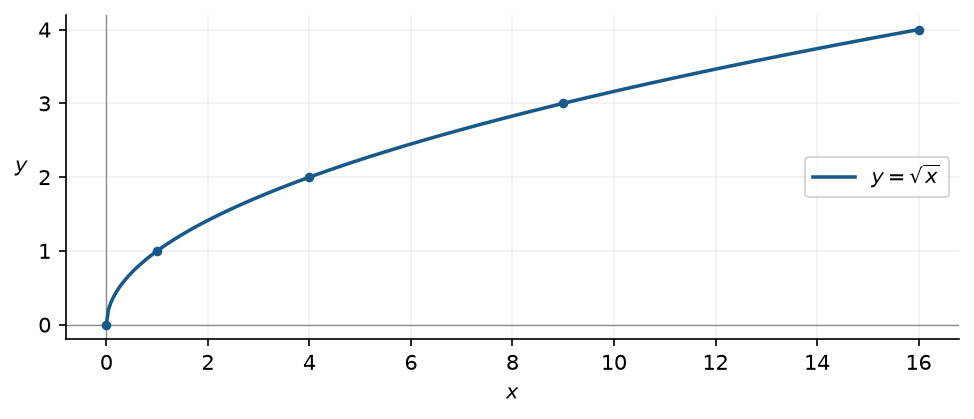
\includegraphics[width=.84\linewidth,height=.38\textheight,keepaspectratio]{figures/C03-EX071-5.png}\end{center}
{\small \field{关联知识}{F04 函数三种表示法、图象与读数（教材帮p.85、86、93、94 / PDF94、95、102、103）}
\field{方法与易错点}{把关键点与定义域一起标到图上，逐区间读交点和上下关系。 易错：将示意图预测当事实；把两曲线交点收进严格不等式；折线漏端点。}
\field{答案依据}{例题原解位置：湘教版教材p.71及题库原图；独立编写可编辑参考解答。答案册此部分主要收练习、习题，不伪造例题答案册位置。}}
